\documentclass{standalone}

\usepackage{tikz}

\begin{document}
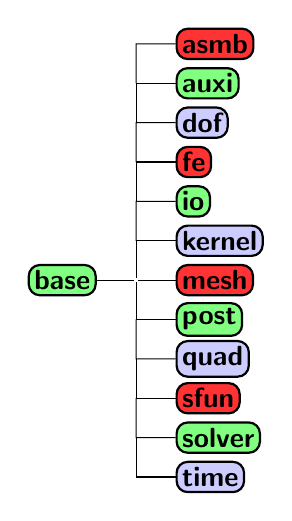
\begin{tikzpicture}
  
  \node[anchor=center,inner sep=-1mm] (X) at (0,0) {};

  % node styles
  \tikzstyle{Box}=[
  anchor=west,
  thick,
  font=\sffamily\bfseries,
  align=center,
  inner sep=0.7mm,
  shape=rectangle,rounded corners,draw]

  \tikzstyle{Label}=[font=\sffamily\bfseries\tiny]

  \draw (X) node[Box,anchor=east,fill=green!50] (I)  at +(-0.5,  0.0) {base};

  \draw (X) node[Box,fill=  red!80] (A1)  at +(0.5, 3.0) {asmb};
  \draw (X) node[Box,fill=green!50] (A2)  at +(0.5, 2.5) {auxi};
  \draw (X) node[Box,fill= blue!20] (A3)  at +(0.5, 2.0) {dof};
  \draw (X) node[Box,fill=  red!80] (A4)  at +(0.5, 1.5) {fe};
  \draw (X) node[Box,fill=green!50] (A5)  at +(0.5, 1.0) {io};
  \draw (X) node[Box,fill= blue!20] (A6)  at +(0.5, 0.5) {kernel};
  \draw (X) node[Box,fill=  red!80] (A7)  at +(0.5, 0.0) {mesh};
  \draw (X) node[Box,fill=green!50] (A8)  at +(0.5,-0.5) {post};
  \draw (X) node[Box,fill= blue!20] (A9)  at +(0.5,-1.0) {quad};
  \draw (X) node[Box,fill=  red!80] (A0)  at +(0.5,-1.5) {sfun};
  \draw (X) node[Box,fill=green!50] (AX)  at +(0.5,-2.0) {solver};
  \draw (X) node[Box,fill= blue!20] (AY)  at +(0.5,-2.5) {time};

  \draw (I.east) -- (X);
  \draw (X) -- (A7.west);
  \draw (X) -- ++(0,-0.5) -- (A8.west);
  \draw (X) ++(0,-0.5) -- +(0,-0.5) -- (A9.west);
  \draw (X) ++(0,-1.0) -- +(0,-0.5) -- (A0.west);
  \draw (X) ++(0,-1.5) -- +(0,-0.5) -- (AX.west);
  \draw (X) ++(0,-2.0) -- +(0,-0.5) -- (AY.west);

  \draw (X) -- ++(0,0.5) -- (A6.west);
  \draw (X) ++(0,0.5) -- +(0,0.5) -- (A5.west);
  \draw (X) ++(0,1.0) -- +(0,0.5) -- (A4.west);
  \draw (X) ++(0,1.5) -- +(0,0.5) -- (A3.west);
  \draw (X) ++(0,2.0) -- +(0,0.5) -- (A2.west);
  \draw (X) ++(0,2.5) -- +(0,0.5) -- (A1.west);

\end{tikzpicture}
\end{document}


%%% Local Variables: 
%%% mode: latex
%%% TeX-master: t
%%% End: 
